\documentclass[a4paper, 11pt]{article}
\usepackage{comment} 
\usepackage{fullpage}
\usepackage{amsmath} 
\usepackage{amssymb} 
\usepackage{mathtools}
\usepackage{siunitx}
\usepackage{xfrac}
\usepackage{icomma}
\usepackage[section,below]{placeins}
\usepackage[labelfont=bf,font=small,width=0.9\textwidth]{caption}
\usepackage{subcaption}
\usepackage{graphicx}
\usepackage{grffile}
\usepackage{float}
\floatplacement{figure}{htbp}
\floatplacement{table}{htbp}
\usepackage{booktabs}
\usepackage{hyperref}
\usepackage{pdfpages}
\sisetup{separate-uncertainty=true}

\begin{document}
\noindent
\centerline{\small{\textsc{Michigan State University}}} \\
\large{\textbf{CMSE 823 – Numerical Linear Algebra \hfill Spring 2020 \\
Homework 9}} \\
Alexander Harnisch \\
\noindent\makebox[\linewidth]{\rule{\textwidth}{0.4pt}}

\section*{24.3}
Here are some examples of the resulting plot. Most of the plots turn out to look something like this:
\begin{figure}[H]
  \centering
  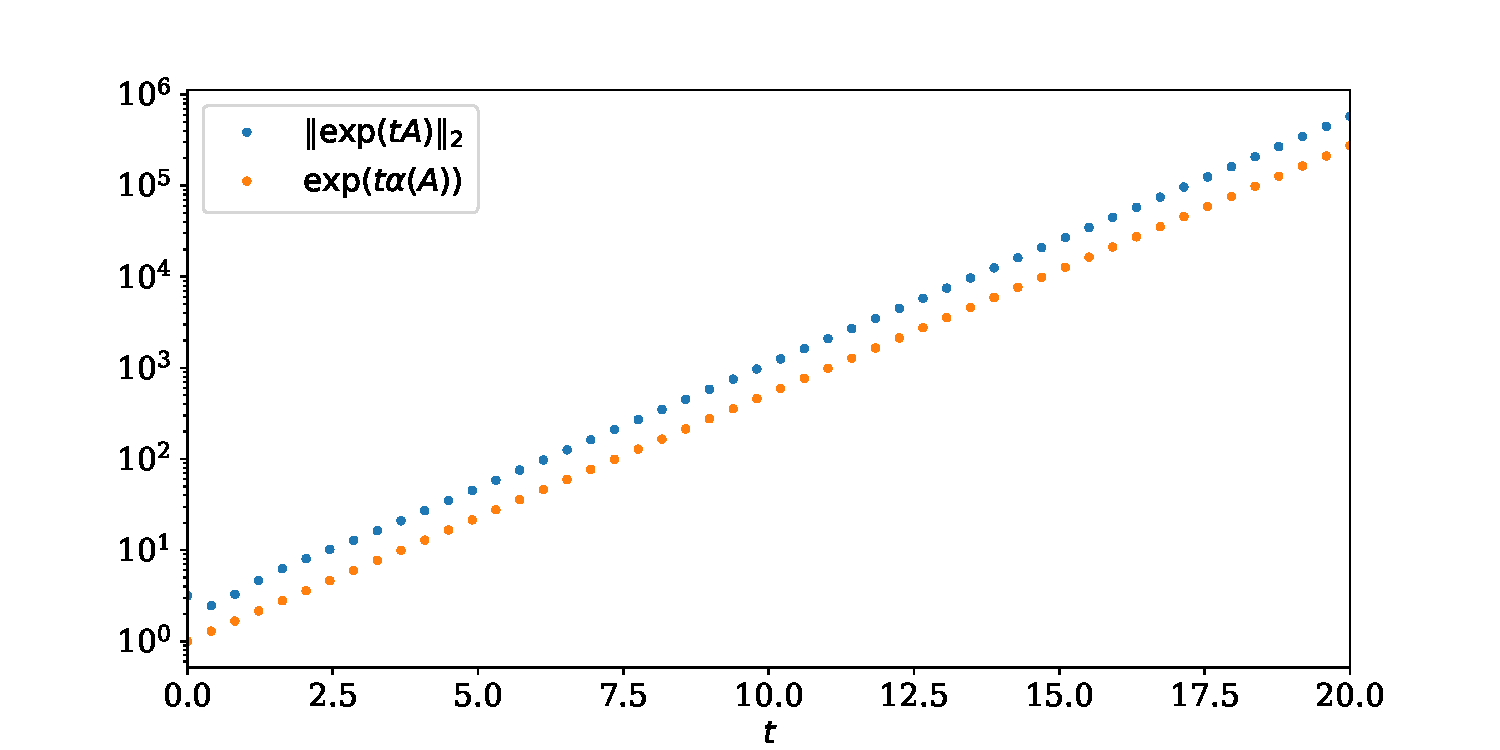
\includegraphics[width=\textwidth]{../24_3/straight_1.pdf}
\end{figure}
\begin{figure}[H]
  \centering
  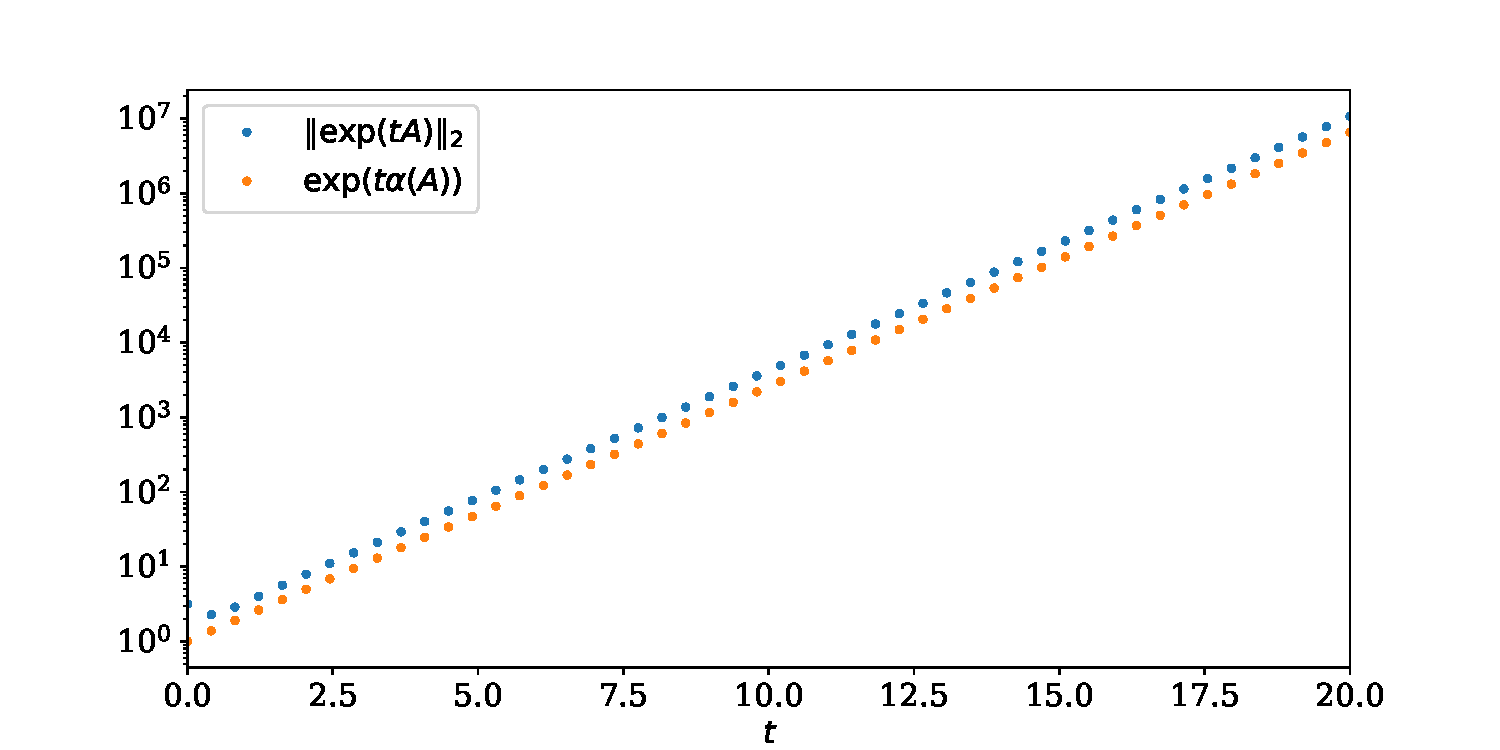
\includegraphics[width=\textwidth]{../24_3/straight_2.pdf}
\end{figure}

However, sometimes oscillations occur:
\begin{figure}[H]
  \centering
  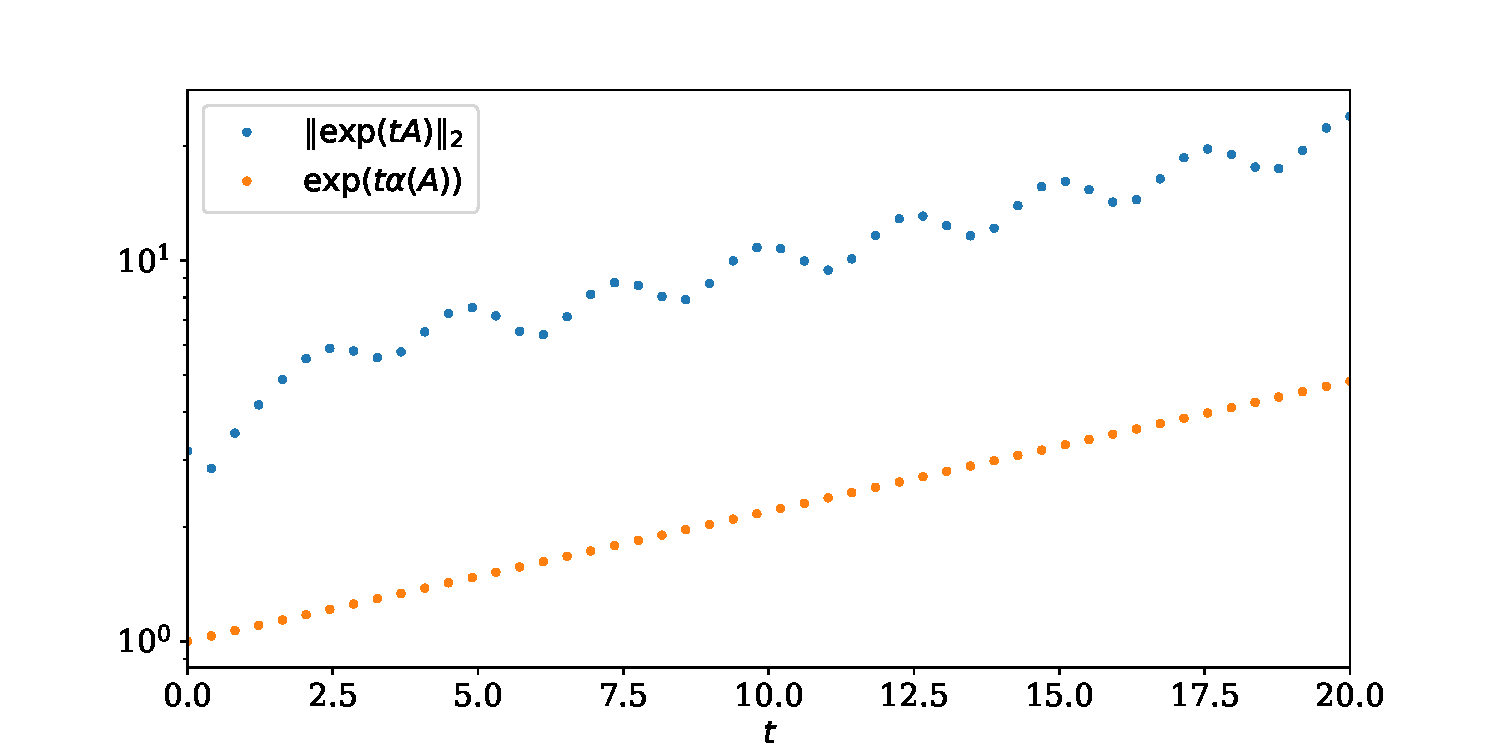
\includegraphics[width=\textwidth]{../24_3/nice_1.pdf}
\end{figure}
\begin{figure}[H]
  \centering
  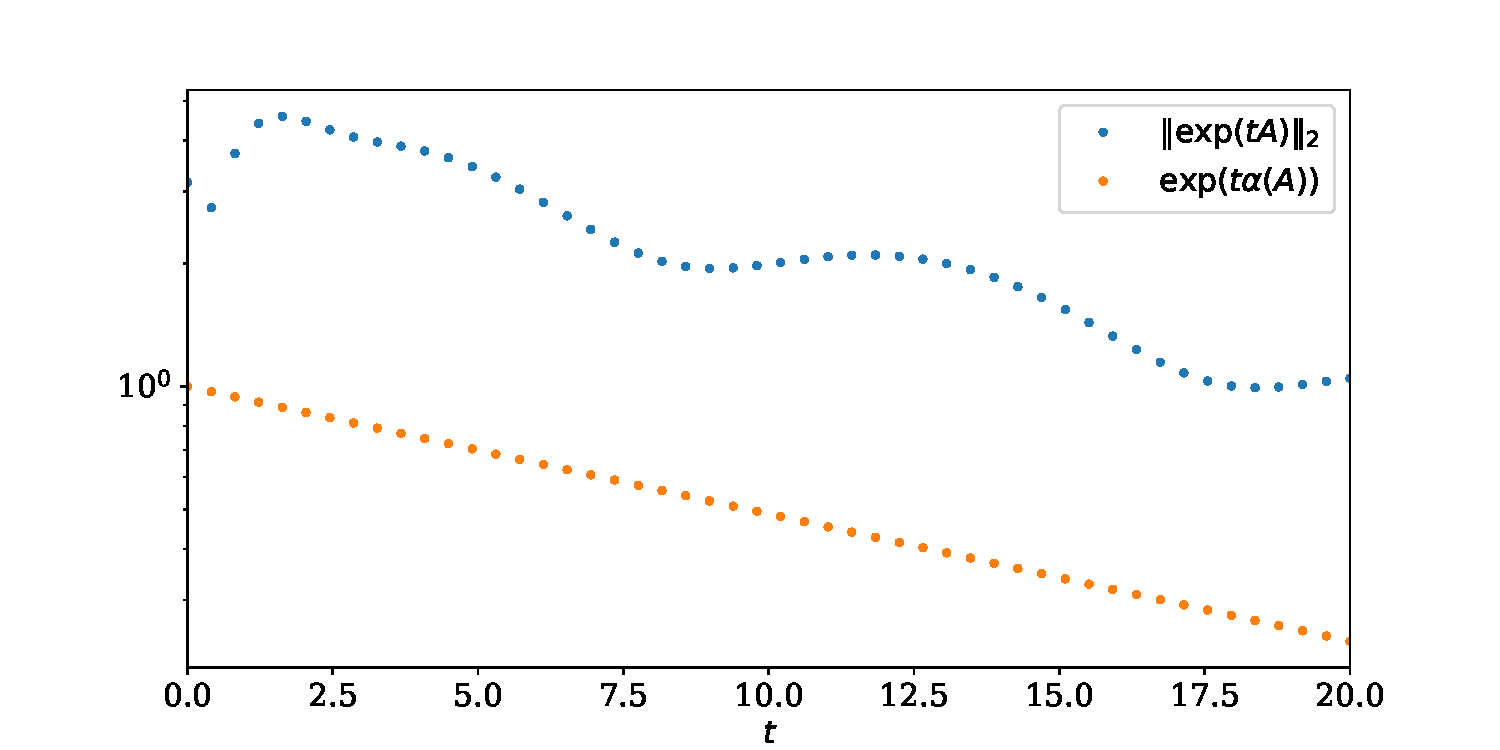
\includegraphics[width=\textwidth]{../24_3/nice_2.pdf}
\end{figure}
\begin{figure}[H]
  \centering
  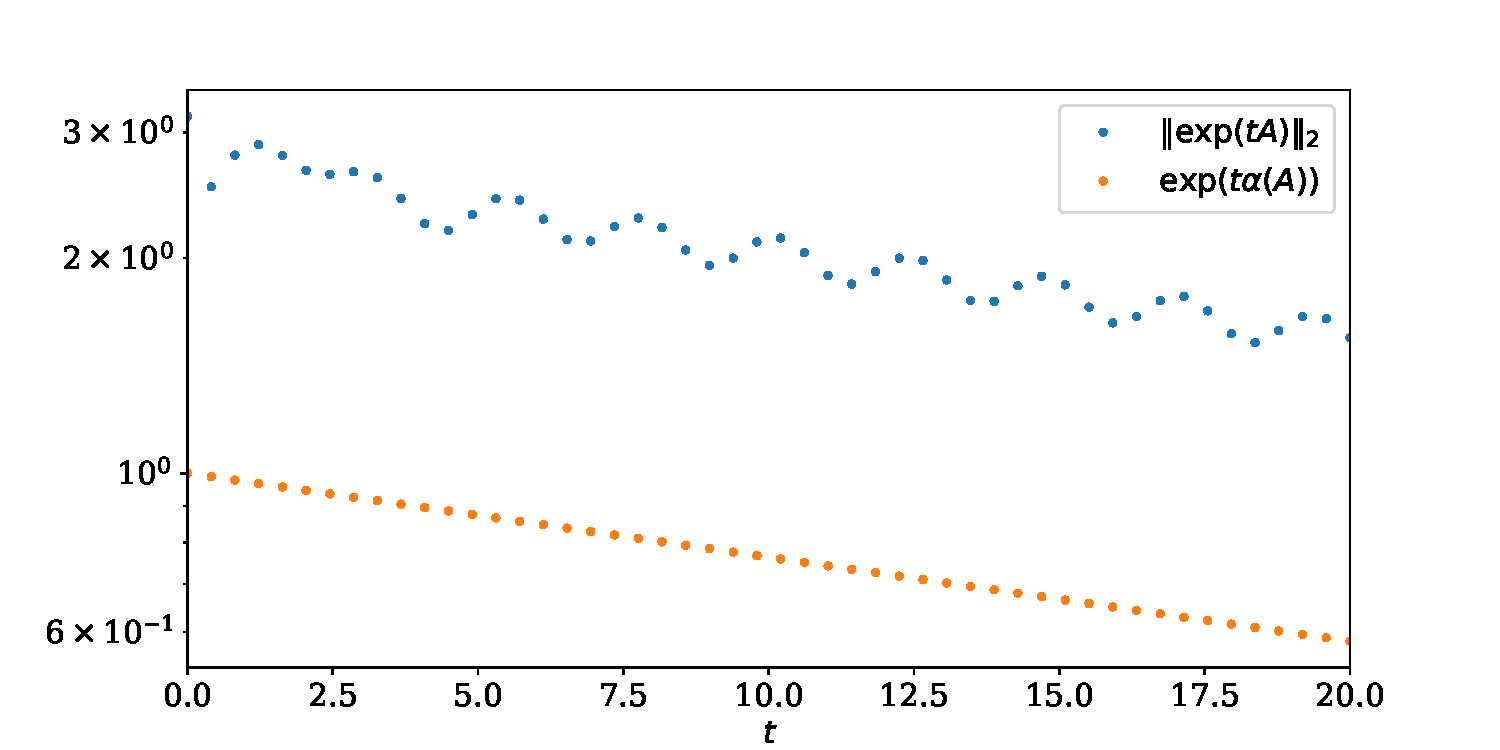
\includegraphics[width=\textwidth]{../24_3/nice_3.pdf}
\end{figure}

And there are also some where it seems to be something in between:
\begin{figure}[H]
  \centering
  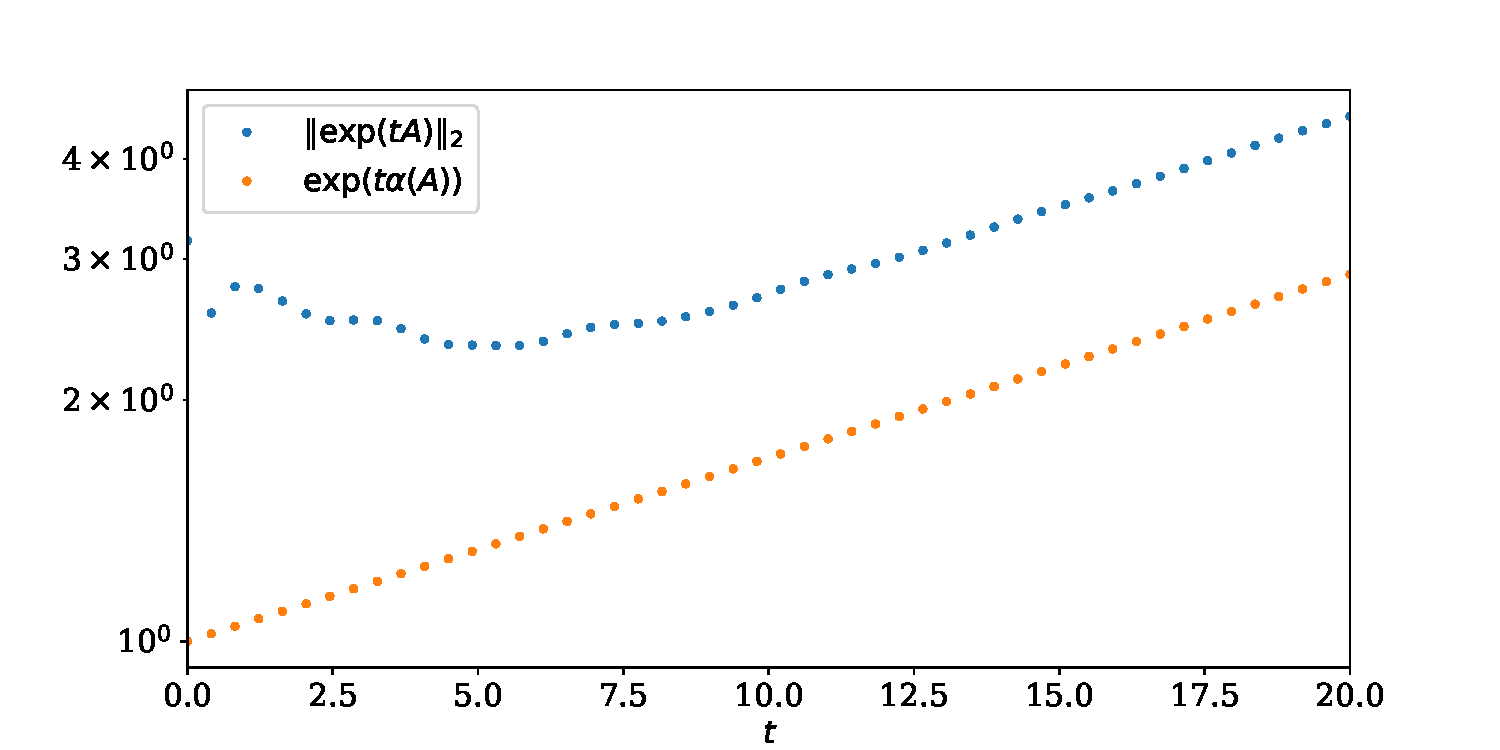
\includegraphics[width=\textwidth]{../24_3/damped.pdf}
\end{figure}
\begin{figure}[H]
  \centering
  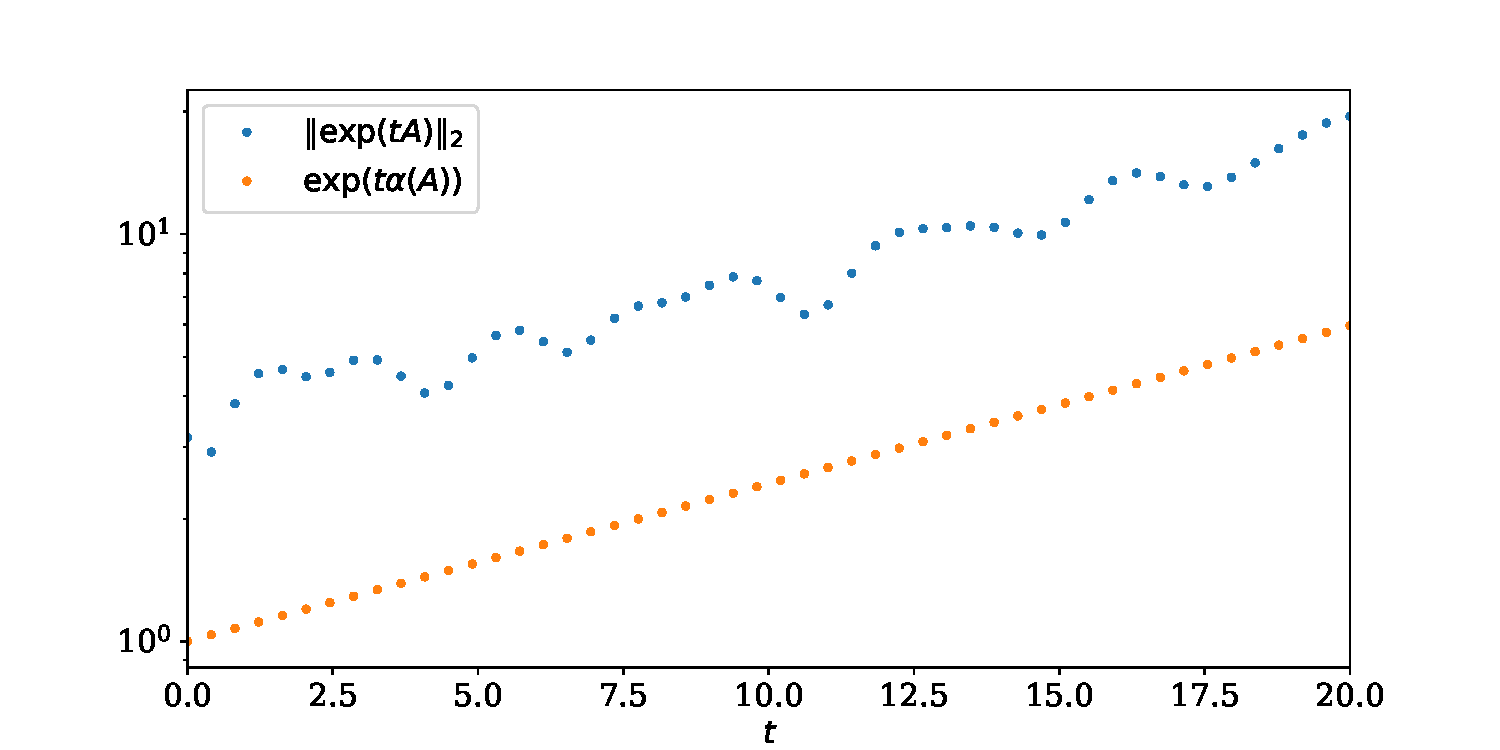
\includegraphics[width=\textwidth]{../24_3/weird.pdf}
\end{figure}

I've played around with this a lot and tried to figure out what leads to the
different outcomes. Sadly I did not come up with anything conclusive. I think
it most likely has something todo with the imaginary parts of the eigenvalues.
Where some combination of more imaginary contribution leads to the
oscillations. However, I did not find a conclusive rule. 


\end{document}
